\documentclass{abntex2}
\usepackage[utf8]{inputenc}
\usepackage{graphicx}
\graphicspath{ {./} }
 
\title{First document}
\author{Douglas Farnsworth \thanks{funded by the ShareLaTeX team}}
\date{\today }


\begin{document}
\maketitle

\begin{abstract}
This is a simple paragraph at the beginning of the 
document. A brief introduction about the main subject.
\end{abstract}

First document. This is a simple example, with no 
extra parameters or packages included.
Give gieve
And the image:
\begin{figure}[h]
    \centering
    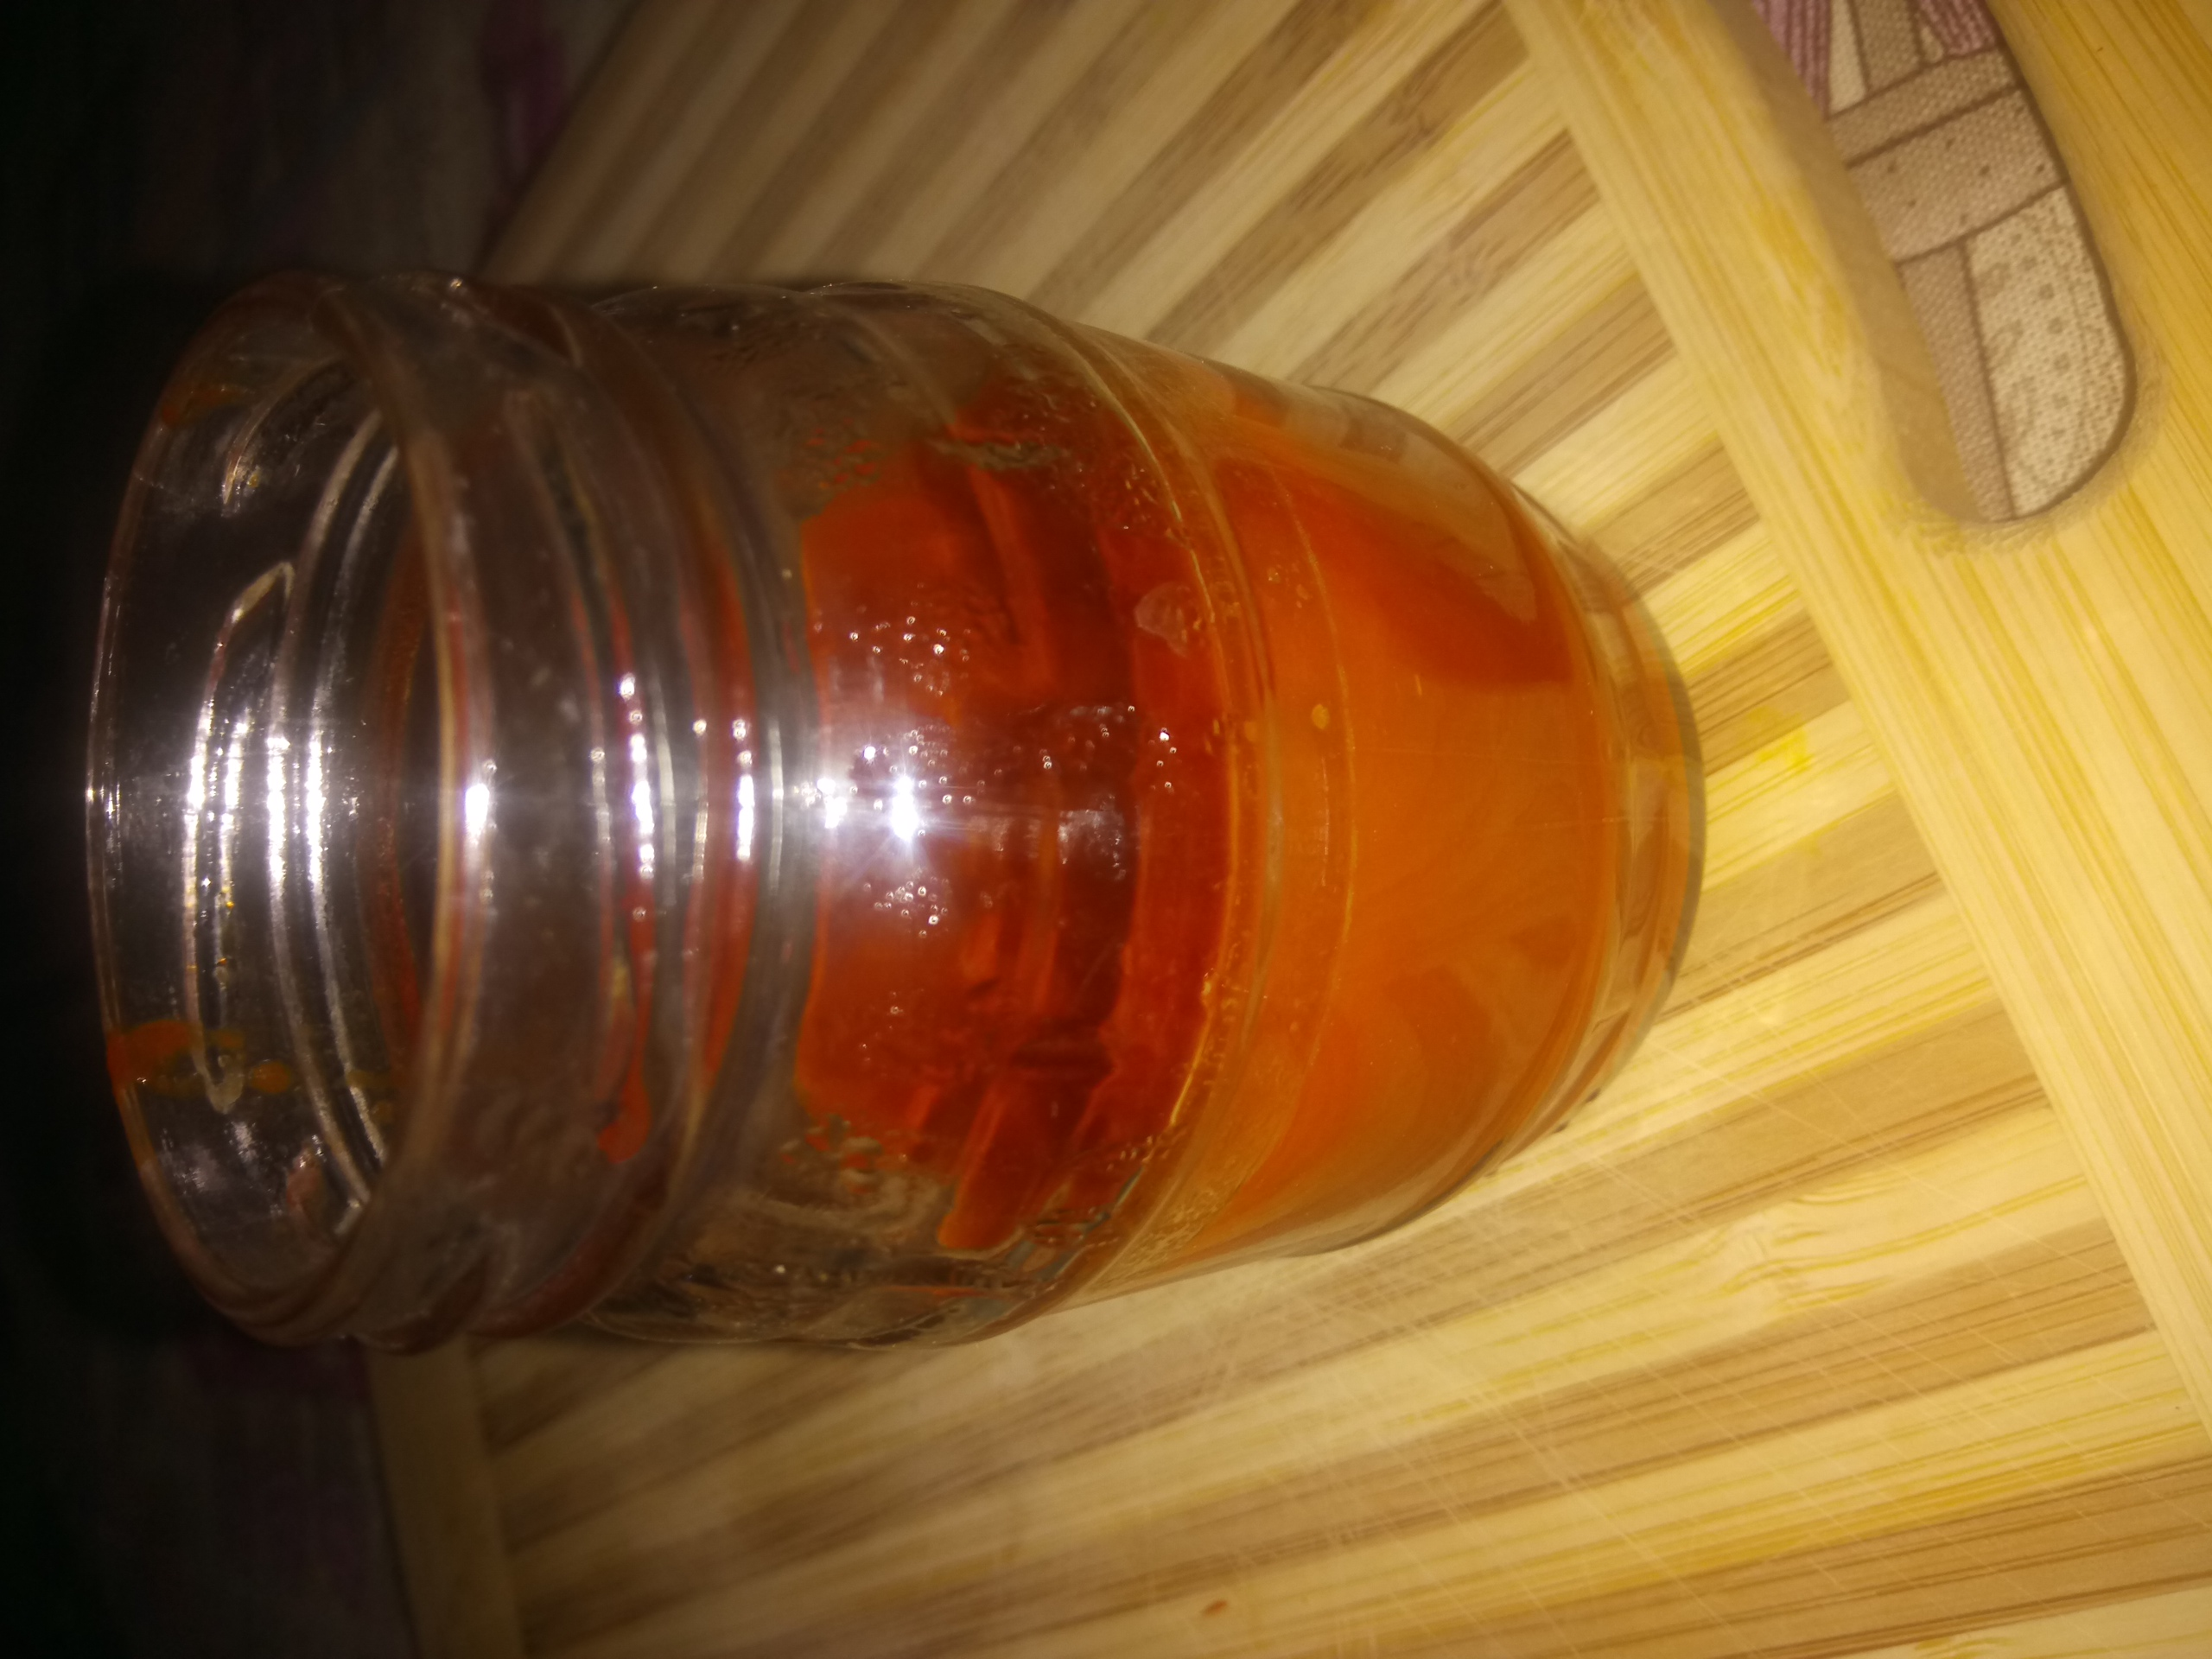
\includegraphics[width=0.25\textwidth]{IMG_20170427_185824}
    \caption{a nice jar}
    \label{fig:jar}
\end{figure}
As you can see in the figure \ref{fig:jar}, the 
function grows near 0. Also, in the page \pageref{fig:jar}



\begin{itemize}
  \item The individual entries are indicated with a black dot, a so-called bullet.
  \item The text in the entries may be of any length.
\end{itemize}





\begin{enumerate}
  \item The individual entries are indicated with a black dot, a so-called bullet.
  \item The text in the entries may be of any length.
\end{enumerate}


\end{document}

